\documentclass[11pt,a4paper]{article}
\usepackage[margin=25mm]{geometry}
\usepackage[T1]{fontenc}
\usepackage[utf8]{inputenc}
\usepackage{lmodern,microtype,amsmath,amssymb,amsthm,mathtools}
\usepackage{booktabs,array,graphicx,xcolor,enumitem,tabularx}
\usepackage[numbers,sort&compress]{natbib}
\usepackage[font=small,skip=5pt]{caption}
\usepackage{hyperref}
\definecolor{plum}{HTML}{6C426B}
\hypersetup{colorlinks=true,linkcolor=plum,citecolor=plum,urlcolor=plum,
 pdftitle={Observable systems with divergent isolated Kalman covariances},
 pdfauthor={Anonymous}}
\numberwithin{equation}{section}
\newtheorem{theorem}{Theorem}[section]
\newtheorem{proposition}[theorem]{Proposition}
\newtheorem{corollary}[theorem]{Corollary}
\newtheorem{lemma}[theorem]{Lemma}
\newtheorem{conjecture}{Conjecture}
\theoremstyle{remark}\newtheorem{remark}[theorem]{Remark}
\newtheorem{finding}[theorem]{Numerical finding}
\newcommand{\T}{^{\mathsf T}}
\newcommand{\one}{\mathbf 1}
\newcommand{\diag}{\operatorname{diag}}
\setlength{\parskip}{4pt}
\setlength{\parindent}{0pt}
\setlist{nosep,leftmargin=*}
\renewcommand{\arraystretch}{1.15}
\title{\textbf{Observable systems with divergent isolated Kalman covariances}\\[6pt]
 \large A counterexample to the isolated Kalman filtering convergence conjecture}
\author{Anonymous\thanks{Text released under CC0~1.0; code under the MIT licence.
 See the accompanying reproducibility package,
 \href{https://doi.org/10.5281/zenodo.23935675}{doi:10.5281/zenodo.23935675}.}}
\date{4 November 2026}
\begin{document}
\maketitle

\noindent\textbf{Status.} Unrefereed candidate. Prepared with AI assistance and checked
internally (AI-assisted review roles and independent recomputation). It has had no human peer
review, and no proof has been formally (machine) verified. Results labelled
\emph{computer-assisted} rest on interval-arithmetic certificates that anyone can re-run;
results labelled \emph{numerical} are evidence, not proofs.

\begin{abstract}
\emph{Plain message.} The isolated Kalman filter (IsoKF) lets nodes of a network update only the
part of a joint covariance that an observation touches, and approximates the rest. Its
authors conjectured that, for any completely observable and controllable system, the
covariance it reports settles to a finite, unique, stable steady state. This is false. We give
a three-node linear system with pairwise observations, observable from a single epoch, for
which the reported variances grow without bound, although every local block the filter uses
stays positive definite and the ordinary Kalman filter stays bounded.

\emph{Results.} A sign-cone and harmonic-mean argument proves exponential divergence for
$A=3I$ and, through a Perron-root comparison, for every connected non-bipartite graph of
pair-sum observations whenever $a^2\ge\rho$ of a schedule matrix. Extra attenuation of
cross-covariances, including deleting them, does not help. Divergence needs unstable
dynamics: for Schur-stable $A$ the reported marginals are always bounded. But very mild
instability is enough. With computer-assisted proofs (outward-rounded interval arithmetic) we
show that for $a^2$ in $(1,1.38]$ the triangle has an invariant region in which variances grow
like $a^{2k}$, reached from the prior $10^{12}I$ at eight certified values of $a^2$ down to
$1+10^{-8}$. At $a^2=21/20$ the prior $I$ provably converges to a bounded fixed point while
$10^{12}I$ diverges, so there is no globally attracting steady covariance.

\emph{What the failure means.} In high-precision numerical tests of the divergent cases the \emph{actual} estimation
error of the IsoKF estimate stays bounded, even while the reported covariance diverges. The
failure we exhibit is therefore gross pessimism: the reported covariance loses its meaning as
an error measure. It is not divergence of the estimate itself in these tests. We also classify
exactly which overlapping participant groups keep every local block positive definite, and
we give a bounded regime for anchored relative measurements.
\end{abstract}

\tableofcontents

\section{Introduction}\label{sec:intro}

\paragraph{In plain English.}
When several robots or sensors estimate a shared state, a central Kalman filter would keep one
big covariance matrix describing how uncertain every quantity is and how errors are
correlated. That is expensive to communicate. The isolated Kalman filter of Jung, Luft and
Weiss~\citep{JungLuftWeiss2025} saves communication: when an observation involves a few nodes
(the \emph{participants}), only those nodes do a proper update, and every correlation with an
outside node is rescaled by a cheap correction factor. The authors conjectured that this
approximation always settles down when the system is observable and controllable. We show by
explicit example that the reported variances can instead grow without limit, and that, for
very mildly unstable dynamics, whether they settle can depend on the starting prior. In our
tests the estimate itself does not blow up. What fails is the uncertainty the filter reports,
which becomes enormously too pessimistic and therefore useless for gating, fusion or
consistency checks.

\paragraph{The conjecture.} The journal article states, in its concluding section,
\begin{quote}
``The IsoKF paradigm leads to a finite, unique, and stable steady-state covariance
$\Sigma_{ikf}^{\infty}$ if the system is completely observable and controllable. The global
covariance may not be positive semidefinite.'' \citep[Conjecture~1]{JungLuftWeiss2025}
\end{quote}
The earlier dissertation formulation~\citep[printed p.~162]{Jung2023thesis} adds that the
stacked block matrices relating to output-coupled instances are positive semidefinite. Our
main counterexample satisfies that additional clause: every participant block stays positive
definite. The journal admits unstable dynamics explicitly: its discussion of the discrete
algebraic Riccati equation notes that a stable steady-state solution can exist ``even if the
dynamic of the system is unstable''~\citep{JungLuftWeiss2025}. Our examples are therefore
inside the conjecture's stated scope. (A previous draft cited a ``Section~5.1.2'' locator for
this remark; we could not confirm that sub-numbering and have removed it.)

\paragraph{Results at a glance.}
Table~\ref{tab:glance} lists every result, how it is established, and what is only numerical.

\begin{table}[ht]
\centering\small
\caption{Results at a glance. ``Proof'' means a written analytic proof; ``computer-assisted''
means a written argument whose finite hypotheses are checked by a re-runnable
interval-arithmetic certificate; ``numerical'' means evidence only.}
\label{tab:glance}
\begin{tabularx}{\textwidth}{>{\raggedright\arraybackslash}p{0.33\textwidth}>{\raggedright\arraybackslash}X>{\raggedright\arraybackslash}p{0.17\textwidth}}
\toprule
Result & Statement in brief & Status\\
\midrule
Prop.~\ref{prop:stable} & Schur-stable $A$: reported marginals are bounded; divergence needs instability & Proof\\
Thm.~\ref{thm:main} & $A=3I$ triangle of pair sums: $\min_i P_{ii}\ge\frac54(\frac95)^k-\frac14$; central KF $\le 3/4$ & Proof (+ exact check of 4 epochs)\\
Thm.~\ref{thm:graph}, Cor.~\ref{cor:atten} & Any connected non-bipartite pair-sum graph diverges if $a^2\ge\rho(M)$; extra attenuation or deletion does not help & Proof\\
Thm.~\ref{thm:mild} & Triangle, $Q=R=I$, $a^2\in(1,1.38]$: invariant escape region, growth exactly at rate $a^{2}$, $P_k/P_{11}\to 2I-\one\one\T$ & Computer-assisted\\
Cor.~\ref{cor:entry} & Prior $10^{12}I$ enters that region for 8 listed $a^2$ from $1+10^{-8}$ to $1.38$ & Computer-assisted\\
Thm.~\ref{thm:coexist}, Cor.~\ref{cor:nonunique} & $a^2=21/20$: $P_0=I$ converges to a bounded fixed point, $P_0=10^{12}I$ diverges; no globally attracting steady covariance & Computer-assisted\\
Finding~\ref{find:error} & Actual error covariance of the IsoKF estimate stays bounded while the reported one diverges & Numerical (80 digits)\\
Finding~\ref{find:thresh} & Divergence threshold from $P_0=I$ is $a^2\approx1.1225$; deletion variant close to $2+\sqrt5$ (finite-horizon bias unresolved) & Numerical\\
Thm.~\ref{thm:family} & Local blocks always stay positive definite iff distinct participant sets share at most one node & Proof (+ exact witness)\\
Prop.~\ref{prop:anchor} & Anchored full-coordinate relative measurements give bounded marginals & Proof\\
App.~\ref{app:witness}, \ref{app:repair} & Exact singularity witnesses outside the algorithm's domain; a positivity-preserving attenuation that still diverges & Proof (+ exact check)\\
\bottomrule
\end{tabularx}
\end{table}

\paragraph{Reading guide.} Section~\ref{sec:recurrence} fixes the recurrence and compares it
with the published equations. Section~\ref{sec:stable} explains why only unstable dynamics can
diverge. Sections~\ref{sec:counter}--\ref{sec:graph} give the short complete refutation and its
graph extension; a reader who wants only the counterexample can stop there.
Section~\ref{sec:mild} shows that mild instability suffices and that there is no globally
attracting steady covariance. Section~\ref{sec:meaning} reports, as numerical findings, what the divergence means
for the actual estimation error. Sections~\ref{sec:family}--\ref{sec:anchor} separate local
well-posedness from boundedness and identify a safe regime relevant to robotics.
Section~\ref{sec:related} places the work in the decentralised-fusion literature, and
Section~\ref{sec:verif} records verification, software scope and open questions. Two appendices
keep further exact results that lie off the main line.

\paragraph{Contribution and scope.} Generic inconsistency of filters that neglect or
approximate correlations, and communication-dependent estimation limits, are known
(Section~\ref{sec:related}). Our contribution is specific to the IsoKF recurrence: the
analytic divergence theorem and its graph extension, the certified mild-instability and
coexistence results, the exact participant-family classification, and the observation that
in our tests IsoKF's marginal-ratio rule diverges at much milder instability than simply
deleting cross-covariances. No earlier statement of these results was found in a bounded
search (Section~\ref{sec:verif}); this is not proof of priority.

\section{The covariance recurrence}\label{sec:recurrence}

\emph{This section fixes exactly which mathematical recurrence is analysed and shows that it is
the one published in~\citep{JungLuftWeiss2025}.}

Partition the state into finitely many nodes, with node dimensions allowed to differ. Write
$X\succ0$ for positive definite, $X\succeq0$ for positive semidefinite and $X\preceq Y$ when
$Y-X\succeq0$. Let $P$ be a symmetric array of covariance blocks. A prediction is
\begin{equation}\label{eq:pred}
P^- = A P A\T + Q,
\end{equation}
with $A$ and $Q$ block diagonal. For an observation with participant set $U$, write
$B=P[U,U]$, let $H_U$ be its sensitivity matrix and $R\succ0$ its noise covariance. Whenever
$B\succ0$, set
\begin{equation}\label{eq:local}
S=H_U B H_U\T+R,\qquad C=B-BH_U\T S^{-1}H_U B .
\end{equation}
The participant block is replaced by $C$. For $i\in U$ and $j\notin U$ the external cross block
becomes
\begin{equation}\label{eq:ratio}
P_{ij}^{+}=D_iP_{ij},\qquad D_i=C_{ii}B_{ii}^{-1},
\end{equation}
with the transposed block updated accordingly; blocks between two nonparticipants are
unchanged. Equations \eqref{eq:pred}--\eqref{eq:ratio}, without projection, rejection or
numerical regularisation, define the recurrence analysed here.

\paragraph{Fidelity to the published update.} Table~\ref{tab:fidelity} sets the journal's
equations beside ours. The journal's correction factor is the ratio of the participant's
posterior to prior \emph{marginal} covariance; it is not a square-root or Cholesky factor, and
it is applied with the marginal $B_{ii}=\Sigma_{uu}^{(-)}$, not the joint participant block.
Nonparticipants receive zero gain, ``$K_o=0$''~\citep{JungLuftWeiss2025}. For scalar nodes,
as in all our counterexamples, there is no ambiguity of factor order either.

\begin{table}[ht]
\centering\small
\caption{The published isolated update~\citep[eqs.~(47)--(50)]{JungLuftWeiss2025} and the
recurrence used here. $\mathcal P$: participants; $\bar{\mathcal P}$: nonparticipants.}
\label{tab:fidelity}
\begin{tabular}{@{}lll@{}}
\toprule
& Jung, Luft and Weiss (2025) & This paper\\
\midrule
cross term & $\breve\Sigma_{uv}^{(+)}=\Sigma_{uu}^{(+)}(\Sigma_{uu}^{(-)})^{-1}\Sigma_{uv}^{(-)}$, $u\in\mathcal P$, $v\in\bar{\mathcal P}$ \ (48) & $P_{ij}^+=C_{ii}B_{ii}^{-1}P_{ij}$ \ \eqref{eq:ratio}\\
factor & $\Lambda_{uu}=\Sigma_{uu}^{(+)}(\Sigma_{uu}^{(-)})^{-1}$ \ (49) & $D_i=C_{ii}B_{ii}^{-1}$\\
buffers & $B_{S_u}\leftarrow\Lambda_{uu}B_{S_u}$ \ (50) & dense array (see below)\\
participants & joint Kalman update of the stacked participant block & $C$ in \eqref{eq:local}\\
\bottomrule
\end{tabular}
\end{table}

\paragraph{Buffered implementation equals the dense array.} The published algorithm stores each
cross-covariance $\Sigma_{uv}$ in factored form, as a product of per-node correction buffers
that are left-multiplied by $\Lambda_{uu}$ at an update and by the node's transition matrix at
a prediction, and assembles $\Sigma_{uv}$ only when needed. Each of these operations is a left
(or, for the partner node, right) multiplication of the represented block, so the assembled
block obeys exactly the same recursion as the dense entry: $\Sigma_{uv}\mapsto A_u\Sigma_{uv}A_v\T$
at prediction and $\Sigma_{uv}\mapsto\Lambda_{uu}\Sigma_{uv}$ at an update of $u$ alone. For
linear time-invariant models, and in particular $A=aI$, the buffered and dense forms therefore
produce identical arrays; the factorisation is a storage device, not a different approximation.

\paragraph{Three properties.} \emph{Local well-posedness}: each scheduled $B$ and $S$ is positive
definite, so the update can proceed. \emph{Covariance boundedness}: the reported marginals stay
bounded. \emph{Statistical consistency}: the reported covariance relates correctly to the actual
estimation error. None of these should be substituted for another.

\section{Stable dynamics cannot diverge}\label{sec:stable}

\emph{This short section shows that any divergence counterexample must use unstable (or
marginally stable) dynamics, and states what remains open for stable dynamics.}

\begin{proposition}\label{prop:stable}
Assume local well-posedness at every step, block-diagonal $A=\diag(A_i)$ and $Q=\diag(Q_{ii})$.
Then for every node $i$ and epoch $k$,
\[
P_{ii}(k)\preceq A_i^kP_{ii}(0)(A_i^k)\T+\sum_{t=0}^{k-1}A_i^tQ_{ii}(A_i^t)\T .
\]
In particular, if every $A_i$ is Schur stable, all reported marginals are uniformly bounded,
for every observation schedule and every prior.
\end{proposition}

\begin{proof}
A local update gives $C=B-BH_U\T S^{-1}H_UB\preceq B$, hence $C_{ii}\preceq B_{ii}$ for each
participant; nonparticipant marginals are unchanged. Prediction maps $P_{ii}$ to
$A_iP_{ii}A_i\T+Q_{ii}$, a monotone map in the Loewner order. Induction gives the bound, whose
right side converges when $\rho(A_i)<1$.
\end{proof}

Thus the boundedness part of the conjecture holds trivially for stable dynamics, and the
question of a \emph{unique} stable steady state for Schur-stable $A$ is untouched by this paper.
At $a=1$ the bound grows only linearly; Section~\ref{sec:mild} records what is known there.

\section{A completely observable pairwise counterexample}\label{sec:counter}

\emph{This section gives the complete short refutation: one explicit system, two lemmas and a
four-line induction.}

\begin{theorem}[Divergence with three scalar nodes]\label{thm:main}
Consider $x_{k+1}=3x_k+w_k$ on $\mathbb R^3$ with $\operatorname{Cov}(w_k)=I_3$ and independent
initial covariance $P_0=I_3$. At each epoch predict once, then process the scalar observation
channels
\begin{equation}\label{eq:H}
H=\begin{pmatrix}1&1&0\\0&1&1\\1&0&1\end{pmatrix},\qquad R=I_3,
\end{equation}
in the displayed order, each on its two nonzero nodes. Let $P_k$ be the IsoKF array after the
three updates at epoch $k$ and $m_k=\min_i(P_k)_{ii}$. Every pairwise participant block remains
positive definite, every innovation is positive, and
\begin{equation}\label{eq:bound}
m_k\ \ge\ \frac54\Big(\frac95\Big)^k-\frac14\ \longrightarrow\ \infty .
\end{equation}
The system is completely observable, and $(A,Q^{1/2})=(3I,I)$ is controllable. The centralised
Kalman posterior satisfies $P_k^{\mathrm{KF}}\preceq(H\T H)^{-1}=I_3-\frac14\one\one\T$ for
$k\ge1$, so every centralised marginal is at most $3/4$.
\end{theorem}

(Earlier drafts added a deterministic input $u_k=0$ with input matrix $I$ to make input
controllability explicit. Controllability from the process noise suffices for the conjecture,
so the device is dropped.)

\begin{lemma}[An invariant cone]\label{lem:cone}
For scalar nodes write $p_i=P_{ii}$ and $P_{ij}=-c_{ij}$ for $i\ne j$, and consider arrays with
\begin{equation}\label{eq:cone}
p_i>0,\qquad 0\le c_{ij}<\min(p_i,p_j).
\end{equation}
A prediction with $A=aI$, $a>0$, and strictly positive diagonal $Q$ preserves
\eqref{eq:cone}. So does every pair-sum observation $x_i+x_j$ with noise variance $r>0$.
\end{lemma}

\begin{proof}
Prediction maps $c_{ij}\mapsto a^2c_{ij}$ and $p_i\mapsto a^2p_i+Q_{ii}$; strictness is kept
because $a^2c_{ij}<a^2p_i<a^2p_i+Q_{ii}$. For a pair update put $p=p_i$, $q=p_j$, $c=c_{ij}$,
$u=p-c>0$, $v=q-c>0$. Then
\begin{equation}\label{eq:pair}
s=u+v+r>0,\qquad p'=p-\frac{u^2}{s},\quad q'=q-\frac{v^2}{s},\quad c'=c+\frac{uv}{s},
\end{equation}
so $p'-c'=ur/s>0$, $q'-c'=vr/s>0$, $0<p'\le p$ and $0<q'\le q$. For an outside node $\ell$,
$c_{i\ell}'=(p'/p)c_{i\ell}<p'$ and $c_{i\ell}'\le c_{i\ell}<p_\ell$; likewise for $j$. Every
two-node block is positive definite because $c_{ij}^2<p_ip_j$.
\end{proof}

\begin{lemma}[Harmonic lower bound]\label{lem:harm}
Under Lemma~\ref{lem:cone}, a pair-sum update obeys $p',q'\ge pq/(p+q)$.
\end{lemma}

\begin{proof}
From \eqref{eq:pair},
\begin{equation}\label{eq:harm}
p'-\frac{pq}{p+q}=\frac{c\{2pq-c(p+q)\}+p^2r}{(p+q)(p+q-2c+r)}\ge0,
\end{equation}
since $c\le\min(p,q)\le2pq/(p+q)$. Exchange $p$ and $q$ for the other bound.
\end{proof}

\begin{proof}[Proof of Theorem~\ref{thm:main}]
$P_0=I$ satisfies \eqref{eq:cone}, and Lemma~\ref{lem:cone} gives local well-posedness. If all
diagonal entries before the observations are at least $t$, monotonicity of $pq/(p+q)$ gives the
successive lower bounds $(t,t,t)\to(t/2,t/2,t)\to(t/2,t/3,t/3)\to(t/5,t/3,t/5)$ after rows
12, 23, 31. Prediction gives $t=9m_k+1$, so $m_{k+1}\ge(9m_k+1)/5$, and with $m_0=1$ induction
gives \eqref{eq:bound}. $\det H=2$ gives observability from one epoch. For the centralised
filter, $P_k^{\mathrm{KF}}=\{(P_k^{\mathrm{KF},-})^{-1}+H\T H\}^{-1}\preceq(H\T H)^{-1}$ and
$H\T H=I+\one\one\T$.
\end{proof}

Unbounded marginals preclude a finite steady-state covariance, so the example refutes the
universal claim of~\citep[Conjecture~1]{JungLuftWeiss2025}, with only pairwise observation
blocks, all of them positive definite. The bound $9/5$ is loose: exact arithmetic gives
$m_k=2.38,\,14.97,\,114.2,\,982.0$ for $k=1,\dots,4$, a ratio near $8.6$ that approaches the
open-loop rate $a^2=9$; Theorem~\ref{thm:mild}(c) proves rate exactly $a^2$ in a milder range.

\section{A schedule-dependent extension}\label{sec:graph}

\emph{This section turns the mechanism into a criterion for any connected graph of pair-sum
observations and shows that additional cross-covariance attenuation cannot repair it.}

For an observed pair $ij$ let $T_{ij}$ replace entries $i,j$ of a vector by their sum and leave
the others unchanged. For a repeated ordered schedule of $L$ pairs set
$M=T_{i_Lj_L}\cdots T_{i_1j_1}$.

\begin{theorem}[Graph criterion]\label{thm:graph}
Let the union observation graph be connected, $A=aI$ with $a>0$, $Q$ positive diagonal with
$Q\succeq q_*I$, $q_*>0$, the prior positive diagonal, and the observations unit pair sums
$x_i+x_j$ with positive noise variances. Let $\rho=\rho(M)$ with Perron vector $v>0$,
$\min_iv_i=1$. Then $t_k:=\min_iv_i(P_k)_{ii}$ satisfies
\begin{equation}\label{eq:perron}
t_{k+1}\ge\frac{a^2t_k+q_*}{\rho}.
\end{equation}
Hence all marginals diverge if $a^2\ge\rho$: at least exponentially if $a^2>\rho$, at least
linearly if $a^2=\rho$. If the graph is also non-bipartite, the stacked observation matrix has
full column rank, giving a completely observable and controllable counterexample on every such
graph.
\end{theorem}

\begin{proof}
For $z_i=1/p_i$, Lemma~\ref{lem:harm} gives $z^+\le T_{ij}z$ componentwise. The $T_{ij}$ are
nonnegative, so $z^{\mathrm{out}}\le Mz^{\mathrm{in}}$ over a schedule; each $T_{ij}\ge I$ and
contains its edge, so connectedness makes $M$ irreducible with a positive Perron vector. Before
the observations $p_i^-\ge(a^2t_k+q_*)/v_i$, i.e.\ $z_i^-\le v_i/(a^2t_k+q_*)$; multiplying by
$M$ and inverting gives \eqref{eq:perron}. If $Hx=0$ then $x_i=-x_j$ on every edge; an odd
cycle forces $x=0$.
\end{proof}

For the triangle schedule of Theorem~\ref{thm:main},
\[
M=\begin{pmatrix}2&2&1\\1&1&1\\2&2&1\end{pmatrix},\qquad\rho=2+\sqrt5,\qquad v=(\varphi,1,\varphi)\T,\ \ \varphi=\tfrac{1+\sqrt5}{2},
\]
so $a^2\ge2+\sqrt5\approx4.236$ suffices.

\begin{remark}[Scope of Theorem~\ref{thm:graph}]\label{rem:graph}
(i) \emph{Order.} All six orders of the three triangle edges give the same $\rho$: cyclic shifts
give conjugate products ($\rho(XY)=\rho(YX)$), and any order is mapped to any other by relabelling
the nodes. (ii) \emph{Robustness.} $a^2>\rho$ is an open condition, so divergence persists under
small changes of $a$, and the theorem allows every positive choice of noise variances and
diagonal process noise; it does not claim robustness to arbitrary structural perturbations of
the measurements. (iii) \emph{Coefficients.} The theorem is stated for unit pair sums. A row
$\kappa_e(d_ix_i+d_jx_j)$ with $\kappa_e>0$ and positive node weights $d_i$ reduces to it: in the
coordinates $y_i=d_ix_i$, $A=aI$ is preserved, $Q$ stays positive diagonal, $R_e$ becomes
$R_e/\kappa_e^2$, and the recurrence is equivariant under diagonal scaling because the scalar
ratio $D_i$ is scale invariant.
\end{remark}

\begin{corollary}[Attenuation and deletion cannot restore boundedness]\label{cor:atten}
Keep the local update \eqref{eq:local} but allow any adaptive factors $0\le\eta_{i\ell}\le1$ in
$P_{i\ell}^+=\eta_{i\ell}(p_i'/p_i)P_{i\ell}$ for participants $i$ and outside nodes $\ell$. The
conclusions of Theorems~\ref{thm:main} and~\ref{thm:graph} still hold. This includes
$\eta\equiv0$, i.e.\ deleting all external cross-covariances, and the common-factor repair of
Appendix~\ref{app:repair}.
\end{corollary}

\begin{proof}
The participant posterior $p_i'$ depends only on the participant block, so it is unchanged by
$\eta$. The new outside magnitude lies in $[0,(p_i'/p_i)c_{i\ell}]$, so the strict cone
\eqref{eq:cone} is preserved as in Lemma~\ref{lem:cone}. Lemma~\ref{lem:harm} holds for every
$c$ in the cone, so every lower bound applies verbatim.
\end{proof}

Corollary~\ref{cor:atten} is an impossibility result for this class of corrections, not for
decentralised filtering in general. The bound is only sufficient: numerically, deletion is
bounded up to a threshold close to $2+\sqrt5$, while the IsoKF rule itself diverges much earlier
(Finding~\ref{find:thresh}).

\paragraph{Why local validity does not prevent the failure.} The array $E=2I_3-\one\one\T$ has
positive diagonal and every two-node block equals
$\left(\begin{smallmatrix}1&-1\\-1&1\end{smallmatrix}\right)\succeq0$, which annihilates its
pair-sum row. Yet $H$ is invertible, and $E$ has eigenvalues $2,2,-1$. Locally compatible but
globally inconsistent covariance relations let the approximation ignore a globally
informative set of measurements. Theorem~\ref{thm:mild}(d) proves that the normalised array
indeed converges to $E$ in the mild-instability range.

\section{Mild instability suffices, and no steady covariance attracts globally}\label{sec:mild}

\emph{This section shows, with computer-assisted proofs, that divergence does not need strong
instability, and that whether the covariance settles can depend on the prior. Throughout,
$A=aI$, $Q=R=I$ and the triangle schedule of Theorem~\ref{thm:main} are used. Scaling
$P\mapsto P/q$ maps $(Q,R)=(qI,qI)$ to $(I,I)$, so all statements hold for $Q=R=qI$ with every
covariance multiplied by $q$; general $Q\ne R$ is not covered.}

\subsection{Deficit form of the recursion}
On the cone \eqref{eq:cone} define six ordered \emph{deficits} $e_{ij}=p_i-c_{ij}>0$, $i\ne j$,
and let $\ell$ be the third node of $\{i,j\}$.

\begin{lemma}\label{lem:deficit}
Prediction maps $p\mapsto a^2p+1$ and $e\mapsto a^2e+1$. The pair-sum update on $\{i,j\}$ with
$r=1$, writing $u=e_{ij}$, $v=e_{ji}$, $s=u+v+1$, $\lambda_i=u^2/s$, $\lambda_j=v^2/s$, is
\begin{equation}\label{eq:deficit}
p_i'=p_i-\lambda_i,\quad e_{ij}'=\frac us,\quad
e_{i\ell}'=\Big(1-\frac{\lambda_i}{p_i}\Big)e_{i\ell},\quad
e_{\ell i}'=e_{\ell i}+\Big(1-\frac{e_{i\ell}}{p_i}\Big)\lambda_i,
\end{equation}
and symmetrically for $j$; all other quantities are unchanged. Moreover
$e_{12}-e_{21}+e_{23}-e_{32}+e_{31}-e_{13}=0$ for every array.
\end{lemma}

\begin{proof}
The first two formulas are \eqref{eq:pair} with $p'-c'=u/s$. By \eqref{eq:ratio},
$c_{i\ell}'=(p_i'/p_i)c_{i\ell}$, so $e_{i\ell}'=(p_i'/p_i)e_{i\ell}$ and
$e_{\ell i}'=p_\ell-c_{i\ell}'=e_{\ell i}+(c_{i\ell}/p_i)\lambda_i$ with
$c_{i\ell}/p_i=1-e_{i\ell}/p_i$. The cycle identity holds since $e_{ij}-e_{ji}=p_i-p_j$.
\end{proof}

The update depends on $p$ only through $e/p$ and $\lambda/p$, so for large $p$ the deficits
evolve almost autonomously. Our certificates use \eqref{eq:deficit} with $e_{13}$ eliminated by
the cycle identity; computing deficits as differences of large numbers, or iterating without
the identity, produces spurious numerical modes.

\subsection{Large priors diverge under mild instability}
\paragraph{Certificate C1.} The range $a^2\in[1,1.38]$ is split into 190 intervals $I_m$ of
width $1/500$. For each $m$ a box $B_m\subset\mathbb R^5$ of radius $0.006$ in the deficit
coordinates $(e_{12},e_{21},e_{23},e_{32},e_{31})$ is given. With $\theta_i=1/p_i$, the
certificate verifies in outward-rounded interval arithmetic, for every $a^2\in I_m$ and every
value of each $\theta_i\in[0,\bar\theta]$, where $\bar\theta\ge10^{-6}$ is the upper endpoint of an outward-rounded enclosure of $10^{-6}$ (each occurrence independently): (1) $F^4(B_m)\subset
\operatorname{int}B_m$, where $F$ is one epoch of \eqref{eq:deficit}, using a mean-value form
whose interval Jacobian is propagated by the chain rule and intersected with naive interval
evaluation; (2) every innovation within each epoch is positive, and all enclosed deficits, including $e_{13}$, are positive at each epoch end (positivity within an epoch follows from Lemma~\ref{lem:cone});
(3) in each of the four epochs each node's total loss $\Lambda_i$ over its two updates obeys
$L_m^-\le\Lambda_i\le L_m$, with $\max_mL_m\le3.1717$ and $L_1^-\ge2.0104$ on $I_1=[1,1.002]$.
The mean-value form is valid because, with the realised $\theta$-values along a true
trajectory held fixed, the epoch map is $C^1$ in $(x,a^2)$ on the convex set $B_m\times I_m$.

\begin{theorem}[Mild-instability divergence; computer-assisted]\label{thm:mild}
Let $Q=R=I$, $a^2\in(1,1.38]$, $a^2\in I_m$, and
$\pi_a=\max\{10^6,(L_m-1)/(a^2-1)\}$. Suppose that at some epoch end $k_0$ the IsoKF array lies
in the cone \eqref{eq:cone}, has deficits in $B_m$ and has $\min_ip_i\ge\pi_a$. Then for all
$k\ge k_0$:
\begin{enumerate}[label=(\alph*)]
\item every local block and innovation stays positive definite, and the deficits at epochs
$k_0+4n$ lie in $B_m$;
\item $p_i(k)-\pi_a\ge a^{2(k-k_0)}(p_i(k_0)-\pi_a)$ and
$p_i(k)\le a^{2(k-k_0)}\big(p_i(k_0)+\frac1{a^2-1}\big)$;
\item if $\min_ip_i(k_0)>\pi_a$, then $\kappa=\lim_ka^{-2k}p_i(k)$ exists, is positive and is the
same for all three nodes, and $p_i(k)=\kappa a^{2k}(1+O(a^{-2k}))$;
\item under the strict inequality in (c), $a^{-2k}P_k\to\kappa E$ with $E=2I_3-\one\one\T$; equivalently $P_k/(P_k)_{11}\to E$, an
indefinite array whose principal block on each observed pair annihilates that pair's local observation row.
\end{enumerate}
\end{theorem}

\begin{proof}
(a),(b) by induction over blocks of four epochs. At a block start with deficits in $B_m$ and
$\min p\ge\pi_a$: after prediction $p_i\ge a^2\pi_a+1$, and after any part of the epoch's
losses $p_i\ge a^2\pi_a+1-L_m\ge\pi_a\ge10^6$ since $(a^2-1)\pi_a\ge L_m-1$. So every realised
$\theta_i\in[0,10^{-6}]$ and the state stays in the certified enclosures, where losses are at
most $L_m$ and denominators are positive. Hence $p_i(k+1)\ge a^2p_i(k)+1-L_m$, i.e.\
$p_i(k+1)-\pi_a\ge a^2(p_i(k)-\pi_a)$. By C1(1) the next block starts in $B_m$; positivity is
Lemma~\ref{lem:cone}. The upper bound uses $\Lambda_i\ge0$.
(c) $a^{-2(k+1)}p_i(k+1)=a^{-2k}p_i(k)+a^{-2(k+1)}(1-\Lambda_i(k))$ with $|1-\Lambda_i|\le
\max(1,L_m)$, so the limit exists with error $O(a^{-2k})$ and, by (b), is at least
$a^{-2k_0}(p_i(k_0)-\pi_a)>0$. The limits coincide because $|p_i-p_j|=|e_{ij}-e_{ji}|$ is
bounded on the certified hull.
(d) $c_{ij}=p_i-e_{ij}$ with $e$ bounded.
\end{proof}

\begin{corollary}[Entry from a positive definite prior; computer-assisted]\label{cor:entry}
Certificate C2 is an outward-rounded interval simulation (60 digits) of the recursion from
$P_0=10^{12}I$. It verifies the hypotheses of Theorem~\ref{thm:mild}, with $\min p>\pi_a$
strictly (lower interval endpoints compared exactly with the rational $\pi_a$), at epoch $k_0$ for
\begin{gather*}
a^2\in\{1+10^{-8},\ 1+10^{-6},\ 1.001,\ 1.01,\ 21/20,\ 1.1,\ 1.2,\ 1.38\},\\
k_0\in\{29,29,29,29,31,32,35,43\}\ \text{respectively}.
\end{gather*}
For each of these values, $P_0=10^{12}I$ (and $10^{12}qI$ when $Q=R=qI$) gives
$(P_k)_{ii}\sim\kappa a^{2k}\to\infty$ and $P_k/(P_k)_{11}\to E$. The same holds on some open
neighbourhood of $10^{12}I$, because $P_0\mapsto P_{k_0}$ is continuous (finitely many steps
with positive innovations and marginals) and the hypotheses at $k_0$ are strict inequalities.
\end{corollary}

\paragraph{Exactly what is and is not proved here.} The invariant escape region is certified for
\emph{every} $a^2\in(1,1.38]$, but entry from an explicit prior is certified only at the eight
listed values; a uniform entry argument through the $O(\log c)$-epoch transient was not
obtained, and the neighbourhood in Corollary~\ref{cor:entry} is not explicit. Nothing is
proved here for $a^2\in(1.38,2+\sqrt5)$, which is covered by neither this result nor
Theorem~\ref{thm:graph}. At $a=1$, a trajectory starting in $B_1$ cannot remain indefinitely in the certified regime
$\min_ip_i\ge10^6$: while it does, C1 gives $\Lambda_i\ge2.0104$, so each marginal decreases by at
least $1.01$ per epoch. Global boundedness at $a=1$ is not established here.

\subsection{Coexistence: a bounded and a divergent trajectory}

\begin{theorem}[Bounded trajectory at $a^2=21/20$; computer-assisted]\label{thm:coexist}
Let $a^2=21/20$, $Q=R=I$, $P_0=I$. Then $P_k$ converges to a fixed point $P_*$ of the epoch map.
The fixed point lies in the certificate box $B_{\mathrm{cert}}$ (centre recorded to 25 digits, radius $10^{-6}$ in each
coordinate; exact endpoints in the certificate output), and hence in the outward-rounded box
\[
\begin{aligned}
p_1&\in[1.4923145,1.4923166], & p_2&\in[1.6897335,1.6897356], & p_3&\in[1.4282154,1.4282175],\\
c_{12}&\in[1.0011916,1.0011937], & c_{23}&\in[1.0904812,1.0904833], & c_{31}&\in[1.1027373,1.1027394].
\end{aligned}
\]
In particular $\sup_k\max_i(P_k)_{ii}<\infty$. ($P_*$ is itself indefinite: $\one\T P_*\one<0$.)
\end{theorem}

\begin{proof}
Certificate C3 is an interval simulation (250 digits) of \eqref{eq:pred}--\eqref{eq:ratio} in
$(p,c)$ variables from $P_0=I$. Write $B=B_{\mathrm{cert}}$; the larger displayed box is used only to report bounds and is not
claimed to be invariant. C3 shows that $P_{80}$ lies in the interior of $B$, and, by mean-value
enclosures, that $F(B)\subset B$, $F^4(B)\subset\operatorname{int}B$ and $\|D(F^4)\|_\infty\le0.5955<1$
on $B$ (row sums of the interval Jacobian's absolute values computed in interval arithmetic,
upper endpoints used), with all innovations and marginals positive and $B$ inside the cone. By the mean-value theorem $F^4$ is an $\infty$-norm contraction of $B$ into
itself, so it has a unique fixed point $x_*\in B$ attracting all of $B$. Since $F(x_*)\in B$ is
also fixed by $F^4$, $F(x_*)=x_*$. Finally $P_{80+4n+j}=F^j(F^{4n}(P_{80}))\to F^j(x_*)=x_*$
for $j=0,\dots,3$.
\end{proof}

\begin{corollary}[No unique globally attracting steady covariance]\label{cor:nonunique}
At $a^2=21/20$ with $Q=R=I$, the prior $P_0=I$ gives a bounded convergent covariance
(Theorem~\ref{thm:coexist}), while $P_0=10^{12}I$, and every prior in an open neighbourhood of
it, gives marginals growing like $\kappa(21/20)^k$ (Theorem~\ref{thm:mild},
Corollary~\ref{cor:entry}). The centralised Riccati recursion for the same system converges
from every $P_0\succeq0$ to the unique stabilising solution, because $(A,H)$ is observable and
$(A,Q^{1/2})$ is controllable~\citep{ChanGoodwinSin1984}.
\end{corollary}

So the conjecture's ``unique, stable'' steady covariance fails to attract globally even where small priors do not diverge,
at an instability of only $5\%$ in variance per epoch. For $a^2\in\{1+10^{-8},1+10^{-6},1.001,
1.01\}$ the divergent prior is certified; the bounded trajectory from $P_0=I$ at those values is
numerically convergent but not separately certified. Figure~\ref{fig:coexist} shows the two
behaviours.

\begin{figure}[ht]
\centering
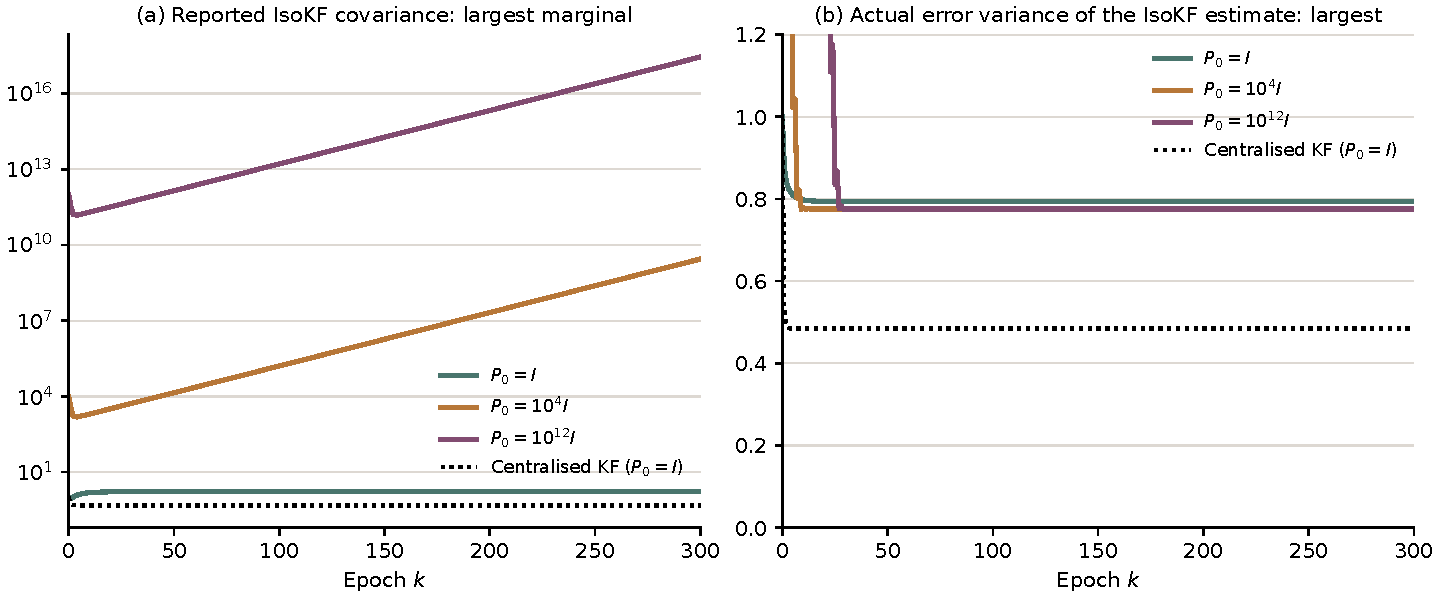
\includegraphics[width=\textwidth]{figures/coexistence.pdf}
\caption{Triangle schedule, $a^2=21/20$, $Q=R=I$, epochs $0$--$300$, computed with 150-digit
decimal arithmetic. (a) Largest reported IsoKF marginal for three priors (logarithmic scale):
$P_0=I$ settles (proved, Theorem~\ref{thm:coexist}); $P_0=10^{12}I$ grows like $1.05^k$ (proved,
Corollary~\ref{cor:entry}); $P_0=10^4I$ also grows (numerical only). Dotted: centralised Kalman
filter. (b) Largest variance of the \emph{actual} error of the IsoKF estimate for the same
priors (linear scale; numerical, Finding~\ref{find:error}): it stays below $0.8$ in all three
cases although the reported variance in (a) reaches $10^{17}$.}
\label{fig:coexist}
\end{figure}

\section{What the divergence means: numerical findings}\label{sec:meaning}

\emph{This section is numerical. It answers two practical questions: does the IsoKF estimate
itself go wrong, and how unstable must the system be? None of it is used in any proof.}

\paragraph{Estimator model.} At a pair observation $y=x_i+x_j+v$ the participants update their
estimates with the local gain $K=Bh\T/S=(u,v)\T/s$ computed from the reported block;
nonparticipants keep their estimates ($K_o=0$); prediction gives $\hat x\leftarrow A\hat x$.
The gains are deterministic, so the covariance $\Sigma$ of the true error obeys the exact linear
recursion $\Sigma\leftarrow A\Sigma A\T+Q$, then $\Sigma\leftarrow F\Sigma F\T+KK\T$ with
$F=I-Kh$ embedded in three dimensions, from $\Sigma_0=P_0$. No Monte Carlo is involved; we
evaluate it in 80-digit arithmetic.

\begin{finding}[Bounded actual error, divergent reported covariance]\label{find:error}
In the tested divergent cases the actual error covariance appears to converge to a bounded limit while the
reported covariance diverges (the bounded case $a^2=1.05$, $P_0=I$ is included for comparison). The
computation needs high precision: in double precision the $a^2=9$ error recursion blows up spuriously
through cancellation in $p-c$.

\begin{center}\small
\begin{tabular}{@{}llll@{}}
\toprule
case & reported $\max_iP_{ii}$ & actual error variances (limit) & centralised KF\\
\midrule
$a^2=9$, $P_0=I$ (Thm.~\ref{thm:main}) & $1.0\times10^{190}$ at $k=200$ & $(4.25,\,3.25,\,3.25)$ & $0.678$\\
$a^2=1.05$, $P_0=I$ & $1.690$ (bounded) & $(0.556,\,0.793,\,0.512)$ & $0.485$\\
$a^2=1.05$, $P_0=10^4I$ & $2.9\times10^{45}$ at $k=2000$ & $(0.561,\,0.776,\,0.496)$ & $0.485$\\
$a^2=1.01$, $P_0=10^8I$ & $5.4\times10^{15}$ at $k=2000$ & $(0.556,\,0.765,\,0.493)$ & $0.482$\\
$a^2=2$, $P_0=I$ & $5.1\times10^{149}$ at $k=500$ & $(0.665,\,1.041,\,0.558)$ & $0.542$\\
\bottomrule
\end{tabular}
\end{center}
The gains stay of order one because they depend only on the bounded deficits, and the
asymptotic epoch error-transition matrix has spectral radius below one ($\approx0$ for $a^2=9$,
$0.45$--$0.57$ otherwise).
\end{finding}

\emph{Interpretation.} In these tests the failure is gross pessimism, not estimate divergence:
the reported covariance stops meaning anything as a measure of error, while the estimate keeps
a bounded error. The estimate is nevertheless worse than the centralised one: by up to about $90\%$ per node in
the mild cases and by a factor of about five to six for $a^2=9$. A reported covariance that is
$10^{45}$ times too large is useless for outlier gating, for fusion with other sources, and for
any consistency check, and it would make a downstream consumer ignore the estimate. We have not
proved boundedness of the actual error; the observed limit $(17/4,13/4,13/4)$ for $a^2=9$ is
not derived analytically.

\begin{finding}[Thresholds]\label{find:thresh}
Double-precision runs of $20000$ epochs with bisection tolerance $10^{-4}$ (classification by
convergence, by $\min p>10^{12}$, or by sustained growth; brackets near slow critical dynamics
are resolution-limited) give the following $a^2$-brackets for the onset of divergence on the
triangle with $Q=R=I$:

\begin{center}\small
\begin{tabular}{@{}lll@{}}
\toprule
rule & prior & threshold bracket for $a^2$\\
\midrule
IsoKF \eqref{eq:ratio} & $I$ & $[1.12251,\,1.12256]$\\
IsoKF & $3I$ & $[1.12241,\,1.12246]$\\
IsoKF & $10I$ & $[1.12206,\,1.12211]$\\
IsoKF & $100I$ & $[1.05207,\,1.05212]$\\
IsoKF & $10^4I$ & $[1.00081,\,1.00086]$\\
deletion ($P_{i\ell}^+=0$) & $I$, $10I$ & $[4.2341,\,4.2342]$\\
deletion & $10^4I$ & $[4.2357,\,4.2358]$\\
\bottomrule
\end{tabular}
\end{center}
\end{finding}

For the IsoKF rule the threshold falls towards $1$ as the prior grows, consistent with
Theorem~\ref{thm:mild}, where the required prior size scales like $1/(a^2-1)$. For deletion the
estimates are close to the Perron threshold $2+\sqrt5\approx4.2361$ of Theorem~\ref{thm:graph}, with an
unresolved finite-horizon bias (the brackets do not contain $2+\sqrt5$, and dynamics near the
threshold are very slow). The IsoKF marginal-ratio rule is
thus markedly \emph{less} robust than simply discarding cross-covariances: the divergence is
not merely the generic effect of neglecting correlations, but a property of this rule.

\section{Which participant families are always locally well defined?}\label{sec:family}

\emph{This section separates local well-posedness from boundedness: it classifies exactly
when every local block stays positive definite, which, by Theorem~\ref{thm:main}, still does not
imply convergence.}

Let $\mathcal G$ be a finite family of distinct nonempty participant sets, node dimensions
arbitrary. The admissible cone $\mathcal A_{\mathcal G}$ consists of symmetric arrays whose node
diagonal blocks and principal blocks $P[U,U]$, $U\in\mathcal G$, are positive definite; such an
array need not be globally positive definite.

\begin{theorem}[Participant-family criterion]\label{thm:family}
The following are equivalent.
\begin{enumerate}
\item For every $P\in\mathcal A_{\mathcal G}$, every observation on some $U\in\mathcal G$ with
positive definite noise and every measurement matrix $H_U$ (of any rank, including rows that
do not touch every participant), the update \eqref{eq:local}--\eqref{eq:ratio} preserves
$\mathcal A_{\mathcal G}$.
\item Any two distinct $U,V\in\mathcal G$ satisfy $|U\cap V|\le1$.
\end{enumerate}
Under condition 2, block-diagonal predictions with positive definite node noise preserve
admissibility, so every finite schedule remains well defined.
\end{theorem}

\begin{proof}
\emph{Sufficiency.} Fix an update on $U$; then $0\prec C\preceq B$. A target group $V$ disjoint
from $U$ is unchanged and $V=U$ becomes $C$. If $U\cap V=\{i\}$, write the old block on $V$ as
$\left(\begin{smallmatrix}X&Y\\Y\T&Z\end{smallmatrix}\right)\succ0$ with $X=P_{ii}$, and set
$X^+=C_{ii}$, $F=X^+X^{-1}$. The updated block is
\[
\begin{pmatrix}F&0\\0&I\end{pmatrix}\begin{pmatrix}X&Y\\Y\T&Z\end{pmatrix}\begin{pmatrix}F\T&0\\0&I\end{pmatrix}
+\begin{pmatrix}X^+-X^+X^{-1}X^+&0\\0&0\end{pmatrix},
\]
a positive definite congruence plus a positive semidefinite term ($0\prec X^+\preceq X$).
Predictions act by congruence plus positive noise.

\emph{Necessity.} If distinct groups share two nodes, orient them so $V\setminus U\ne\emptyset$
and pick $a,b\in U\cap V$, $c\in V\setminus U$. On these coordinates take
\[
P_0=\begin{pmatrix}1&0&1/2\\0&1&-1/2\\1/2&-1/2&1\end{pmatrix}\succ0
\]
(leading minors $1,1,1/2$), other coordinates independent with unit variance. Observe
$x_a-x_b$ on $U$ with variance $1/4$:
\[
P_1=\begin{pmatrix}5/9&4/9&5/18\\4/9&5/9&-5/18\\5/18&-5/18&1\end{pmatrix},\qquad\det P_1=-7/162,
\]
so the block on $V$ is no longer positive definite. If $U$ has further participants or node
coordinates, add independent observation rows for them with positive noise; they do not change
$P_1$. This is why condition~1 must allow measurement rows that leave some participants
untouched by the critical row.
\end{proof}

Every pairwise family satisfies condition~2, as do singletons and a single large group. The
obstruction concerns distinct groups sharing two or more nodes; it does not say every such
schedule fails for every prior. With $h=(2,-2,-1)\T$, $P_1h=(-1/18,1/18,1/9)\T$ and
$h\T P_1h=-1/3$, so a further observation on $V$ with noise $1/3$ has zero innovation and a
nonzero gain numerator. In hypergraph language condition~2 says $\mathcal G$ is a
\emph{linear} hypergraph.

\section{A bounded regime with direct anchors}\label{sec:anchor}

\emph{This section identifies where the negative results do not bite, and explains which
measurement models carry the risk in robotics.}

\begin{proposition}[Anchored relative observations]\label{prop:anchor}
Consider node states of equal dimension; each period has one block-diagonal prediction and
finitely many private and pairwise updates, with initially positive definite participant
blocks and positive definite node process noise, and $\|A_i\|_2\le b$, $Q_{ii}\preceq qI$
uniformly. An anchor receives a full-coordinate direct observation every period with noise at
most $r_0I$, and each edge of a fixed connected graph receives a full-coordinate difference
observation $x_i-x_j$ every period with noise at most $rI$; other private or pairwise
observations are allowed. Put $B_0=r_0$, $B_{d+1}=b^2B_d+q+r$. A node at graph distance $d$ from
the anchor has $P_{ii}(k)\preceq B_dI$ at the end of every period $k\ge d+1$. Hence, with $D$ the
largest distance from the anchor, every marginal is bounded by $\max_{d\le D}\{B_d,b^2B_d+q\}I$
for all $k\ge D+1$, and is finite during the initial transient.
\end{proposition}

\begin{proof}
Theorem~\ref{thm:family} gives local positive definiteness. For a pair prior
$\left(\begin{smallmatrix}X&E\\E\T&Y\end{smallmatrix}\right)$ and observation $[I,-I]$ put
$S=X+Y-E-E\T+R\succ0$. Expanding with $X+R-E=S-(Y-E\T)$ gives the exact identity
$X+R-C_{jj}=(X+R-E)S^{-1}(X+R-E\T)\succeq0$, so $C_{jj}\preceq X+R$ without commutativity
assumptions. The anchor's posterior is at most $r_0I$ every period, and later updates only
decrease participating marginals. If a neighbour at distance $d$ has end-of-period bound
$B_dI$, then in the next period it is at most $(b^2B_d+q)I$ until the edge observation, which
bounds the node at distance $d+1$ by $B_{d+1}I$; later observations only decrease it. This
holds for every edge ordering, using the preceding period's bound.
\end{proof}

Full-coordinate pair sums have the same transfer bound (change the sign of one node); more
generally $h_ix_i+h_jx_j$ with $h_j\ne0$ gives $p_j^+\le(h_i/h_j)^2p_i+R/h_j^2$.

\paragraph{What this means for robotics.} Collaborative localisation mostly uses
\emph{differences} (relative poses). An unanchored graph of differences is never observable,
since adding a common offset to all nodes is invisible, so it cannot be a counterexample to the
conjecture; with an anchor, Proposition~\ref{prop:anchor} proves boundedness. The risk lies in
\emph{sum-type or mixed-sign} channels on an odd cycle with no direct anchor. A physical
example is two-way time-of-flight ranging between devices whose unknown internal delays
$b_i$ are estimated as states: each range measurement between devices $i$ and $j$ contains
$b_i+b_j$, so ranging around a triangle of devices gives exactly the pair-sum structure of
Theorem~\ref{thm:main} for the delay states, observable without an anchor. Shared calibration
offsets entering two sensors with the same sign behave in the same way. Our divergence results
additionally require growth ($a>1$) in those states; we do not claim that a specific deployed
system has this property.

\section{Related work}\label{sec:related}

\emph{This section says what is known about filters that approximate or neglect correlations,
and what is specific to the IsoKF recurrence.}

\paragraph{The IsoKF line.} The marginal-ratio cross-covariance correction comes from the
decentralised collaborative localisation of Luft and co-authors~\citep{Luft2016,Luft2018} and
was developed into isolated Kalman filtering in the dissertation~\citep{Jung2023thesis} and the
journal article~\citep{JungLuftWeiss2025}, which also gives the conjecture. Distributed
multi-robot localisation with a decomposed centralised filter goes back at least to
Roumeliotis and Bekey~\citep{RoumeliotisBekey2002}. A forward-citation check of
\citep{JungLuftWeiss2025} on 4 November 2026 found two related citing works: the buffer-driven
decentralised estimator D-GVIO~\citep{DGVIO2026} and the distributed Kalman-like observer of De
Carli and Dimarogonas~\citep{DeCarliDimarogonas2025}. By their titles and abstracts neither
analyses IsoKF covariance convergence; we did not read their full texts.

\paragraph{Consider (Schmidt) filters.} Updating only some states while holding others fixed is
the classical Schmidt--Kalman or consider filter~\citep{Schmidt1966}. Its exact cross-covariance
correction for fixed nonparticipants is $F=CB^{-1}=I-KH$ applied to the whole participant block;
IsoKF replaces it by the block-diagonal marginal ratio $\diag(C_{ii}B_{ii}^{-1})$, which avoids
communicating the participants' joint factor. The full correction lies outside the class of
Corollary~\ref{cor:atten}; we prove no stability statement for it.

\paragraph{Correlation neglect and conservative fusion.} Fusing estimates whose correlation is
ignored can double-count information and become overconfident; covariance
intersection~\citep{JulierUhlmann1997} and split covariance
intersection~\citep{LiNashashibi2012} restore consistency by conservative bounds. IsoKF sits
between these: it keeps an approximate correlation rather than bounding it. Our failure is in
the opposite direction from double counting: the reported covariance becomes far too
pessimistic. Corollary~\ref{cor:atten} shows that the classical remedy of shrinking or deleting
cross-covariances does not restore boundedness for the same models, and
Finding~\ref{find:thresh} shows that deletion is in fact more robust than the IsoKF rule.

\paragraph{Graphical models and limits.} The odd-cycle (non-bipartite) condition echoes known
pathologies of loopy Gaussian belief propagation, whose means are correct at convergence but
whose variances are not~\citep{WeissFreeman2001}. Communication-dependent tracking limits for
networked estimation are studied in~\citep{KhanJadbabaie2011}. Static maximum-determinant
completion~\citep{Georgescu2018} concerns one consistent partial matrix and does not by itself
give an invariant for successive local substitutions.

\section{Verification, software and open questions}\label{sec:verif}

\emph{This section lists how each result was checked, what the software observation does and
does not show, and what remains open.}

\paragraph{Checks.} Exact rational programs check four complete epochs of
Theorem~\ref{thm:main} together with the identities \eqref{eq:pair}--\eqref{eq:harm}, the
schedule matrix and its characteristic polynomial $\lambda(\lambda^2-4\lambda-1)$, the witnesses
of Theorem~\ref{thm:family} and Appendix~\ref{app:witness}, and the anchored identity with
non-commuting blocks. Certificates C1--C3 use outward-rounded interval arithmetic (mpmath 1.3.0).
Every script performs explicit checks that also run under \texttt{python -O} and exits with a
nonzero code on failure; all outputs were regenerated in normal and \texttt{-O} mode and agree
byte for byte. All scripts, certificates and outputs are archived with this paper at
\href{https://doi.org/10.5281/zenodo.23935675}{doi:10.5281/zenodo.23935675}. Figure~\ref{fig:growth} illustrates Theorem~\ref{thm:main}; its infinite-horizon
conclusion follows from the proof, not from the plot.

\begin{figure}[ht]
\centering
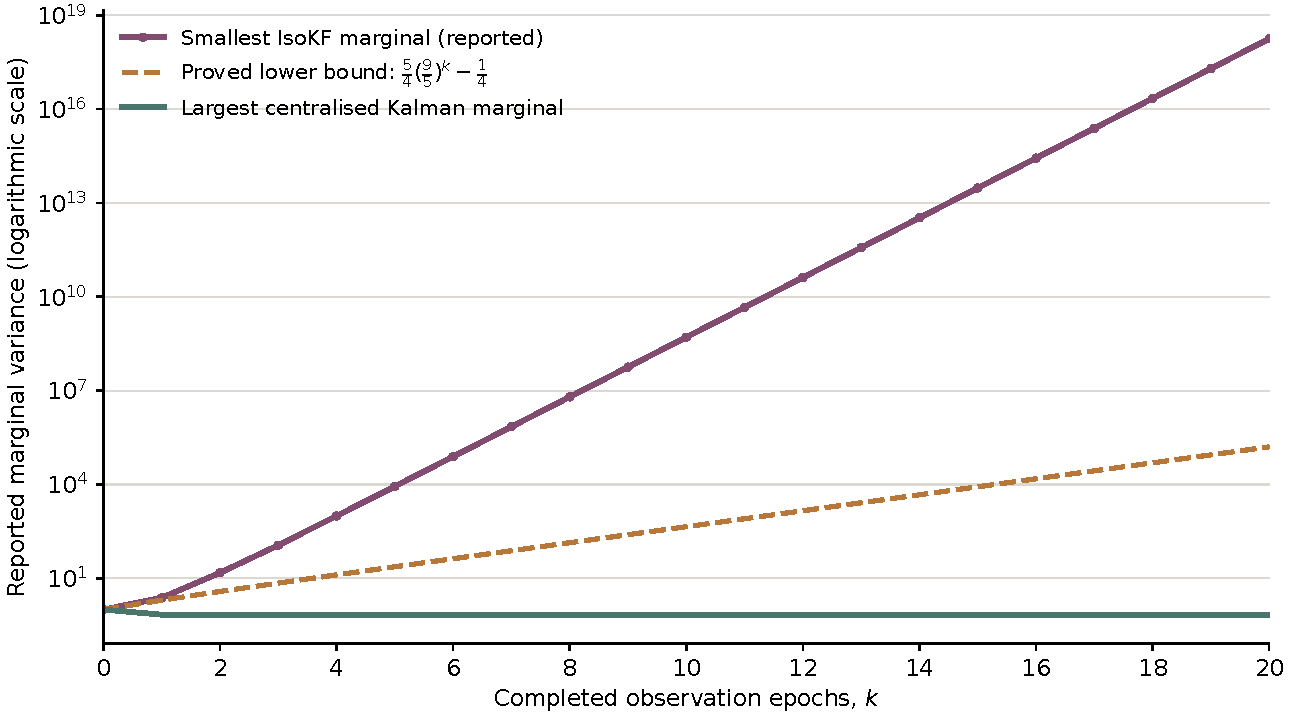
\includegraphics[width=0.82\textwidth]{figures/covariance_growth.pdf}
\caption{System of Theorem~\ref{thm:main} ($A=3I$, $Q=R=P_0=I$), epochs $0$--$20$, logarithmic
scale. Solid purple: the \emph{smallest} reported IsoKF marginal $\min_iP_{ii}$; dashed: the
proved lower bound \eqref{eq:bound}; green: the \emph{largest} centralised Kalman marginal.
Curves computed with 100-digit decimal arithmetic; the bound is analytic.}
\label{fig:growth}
\end{figure}

\paragraph{Software scope.} The official \texttt{ikf\_lib} source was inspected at a pinned
commit~\citep{ikflib}. Its observation handler includes numerical stabilisation, a check that
the participant prior is positive semidefinite, and an optional projection of the participant posterior.
Our pairwise counterexample keeps every participant prior and posterior positive definite, so
the check would not trigger and the projection is inactive; it cannot mask the divergence. We did not
compile or run the library and claim no observed software failure. The observation order is
fixed and repeated, without delays; combining the three rows into one full-state update gives
the ordinary Kalman filter and changes the architecture being tested.

\paragraph{Prior-art search.} Two web engines, arXiv, the publisher's full text of
\citep{JungLuftWeiss2025}, the full 2016 precursor~\citep{Luft2016}, relevant chapters of
\citep{Jung2023thesis}, the software repository and a forward-citation sweep were searched on
1--4 November 2026. The full text of the 2018 journal article~\citep{Luft2018} was not
available to us and was inspected at abstract level only; since~\citep{JungLuftWeiss2025} states
that its correction equals that of Luft et al., a divergence analysis there would bear on this
work. No matching theorem was found in the inspected corpus.

\paragraph{Open questions.}
(i) Entry into the escape region for every $a^2\in(1,1.38]$, and anything proved for
$a^2\in(1.38,2+\sqrt5)$. (ii) The exact divergence threshold from $P_0=I$ (numerically
$a^2\approx1.1225$). (iii) A proof that the actual estimation error stays bounded
(Finding~\ref{find:error}). (iv) Uniqueness of the steady state for Schur-stable $A$ and the
case $a=1$. (v) Other graphs, noise ratios $Q\ne R$, and finite-precision behaviour of the
software.

\section{Conclusions}\label{sec:conc}

The convergence conjecture for isolated Kalman filtering is false. A three-node system with
pairwise sum observations, observable from one epoch and controllable through its process noise,
has reported variances that provably grow without bound while every local block stays
positive definite and the centralised filter stays bounded. Divergence needs instability, but
only a little: computer-assisted proofs show growth at the open-loop rate for large priors at
instabilities down to $a^2=1+10^{-8}$, and coexistence of a bounded and a divergent trajectory
at $a^2=21/20$, so there is no globally attracting steady covariance either. In the tested divergent
cases the actual error of the IsoKF estimate stayed bounded (numerical finding). The practical failure is therefore that the reported
covariance becomes grossly pessimistic and loses its meaning, not that the estimate diverges.
Local positive definiteness is guaranteed exactly when participant groups overlap in at most
one node, and anchored relative measurements remain safe.

\appendix

\section{Exact failures outside the algorithm's domain}\label{app:witness}

\emph{This appendix is outside the domain of the IsoKF update: it shows how unrestricted group
processing can reach an array where the next update is undefined or meaningless. It is not
needed for, and is not part of, the refutation.}

Take $A=2I_3$, $Q=I_3$, $P_0=I_3$ and process $h_1=(1,-1,0)$, $h_2=(0,1,-1)$, $h_3=(2,-3,2)$ with
noise variances $1,1,155/132$; the stacked matrix has determinant one. After prediction and
the first two observations,
\[
P_*=\begin{pmatrix}30/11&25/16&0\\25/16&15/8&25/16\\0&25/16&205/96\end{pmatrix},
\qquad\det P_*=-\frac{257375}{270336}.
\]
Every two-node block is positive definite, but the prior for the three-participant observation
has left the positive definite domain of Section~\ref{sec:recurrence}; what follows is
unchecked algebraic continuation of \eqref{eq:local}. Here $P_*h_3\T=(135/176,5/8,-5/12)\T$ and
$h_3P_*h_3\T=-155/132$, so the third innovation is exactly zero with nonzero numerator. With
$R_3=5/4$ the innovation is $5/66>0$ but the marginals become $(-645/128,-105/32,-5/32)$. Writing
$R_3=155/132+\varepsilon$ gives $S=\varepsilon$ and new diagonal entries
$(P_*)_{ii}-(P_*h_3\T)_i^2/\varepsilon$; all three are negative exactly when
$0<\varepsilon<10/123$, i.e.\ $155/132<R_3<2265/1804$. These strict inequalities persist under
small perturbations within the fixed participant architecture.

\section{A positivity-preserving attenuation that still diverges}\label{app:repair}

\emph{This appendix records a standard Schur-complement consequence. We claim no novelty for
the matrix criterion and infer no stability or consistency from it.}

Suppose a participant update replaces $B\succ0$ by $C\succ0$, leaves the nonempty nonparticipant
block $Z$ unchanged and replaces the cross block $X$ by $FX$. The map
$\left(\begin{smallmatrix}B&X\\X\T&Z\end{smallmatrix}\right)\mapsto
\left(\begin{smallmatrix}C&FX\\X\T F\T&Z\end{smallmatrix}\right)$ preserves positive
semidefiniteness for every globally positive semidefinite completion $(X,Z)$ if and only if
\begin{equation}\label{eq:repair}
FBF\T\preceq C.
\end{equation}
\emph{Sufficiency:} add $\diag(C-FBF\T,0)$ to a congruence of the original array.
\emph{Necessity:} one outside coordinate suffices. For a vector $x$ take cross column $x$ and
outside variance $x\T B^{-1}x$; this completion is positive semidefinite (not definite). Its
image must be positive semidefinite, and the Schur-complement condition gives
$x\T F\T C^{-1}Fx\le x\T B^{-1}x$ for all $x$, i.e.\ $F\T C^{-1}F\preceq B^{-1}$, equivalent to
\eqref{eq:repair} via $\|C^{-1/2}FB^{1/2}\|\le1$. If strictly positive definite test completions
are wanted, use $Z+\epsilon I$; the images are positive definite for each $\epsilon>0$, and
letting $\epsilon\downarrow0$ the limit is positive semidefinite because the positive
semidefinite cone is closed.

For IsoKF put $D=\diag_{i\in U}(C_{ii}B_{ii}^{-1})$. The largest common factor
$\alpha\in[0,1]$ with $F=\alpha D$ satisfying \eqref{eq:repair} is
\[
\alpha_*=\min\Big\{1,\ \lambda_{\max}\big(C^{-1/2}DBD\T C^{-1/2}\big)^{-1/2}\Big\}.
\]
It uses only participant information; applying $\alpha_*D_i$ preserves global positive
definiteness under any schedule from a globally positive definite start, and so prevents the
failures of Appendix~\ref{app:witness}. But by Corollary~\ref{cor:atten} it still diverges on
the examples of Theorems~\ref{thm:main}--\ref{thm:graph}: global positivity and boundedness are
separate requirements. The full Schmidt correction $F=CB^{-1}$ also satisfies \eqref{eq:repair},
since $CB^{-1}C\preceq C$, but lies outside Corollary~\ref{cor:atten}.

\bibliographystyle{plainnat}
\bibliography{refs}

\end{document}
